\section{69 - MAT - AN 1.3, AN 4.3, FA 5.6  - Sonnenstrom in Österreich - Matura 2015/16 2. Nebentermin}

\begin{langesbeispiel} \item[0] %PUNKTE DES BEISPIELS
	
In einer Fotovoltaikanlage wird Sonnenstrahlung mithilfe von Solarzellen in elektrische Energie umgewandelt und somit "`Sonnenstrom"' erzeugt. In Österreich arbeiten Solarmodule am effizientesten, wenn sie nach Süden ausgerichtet sind.\leer

Man unterscheidet dabei die sogenannten aufgeständerten Systeme, bei denen die Module entsprechend dem Einfall der Sonnenstrahlung bewegt werden können, und die kostengünstigeren Systeme mit einer dachparallelen Montage.\leer

Überschüssiger Strom kann ins öffentliche Stromnetz eingespeist werden, was die Stromkosten eines Haushalts weiter verringert.\leer

Die nachstehende Grafik zeigt die Zunahme an Sonnenstrom seit dem Jahr 2000.
\begin{center}
	\resizebox{0.8\linewidth}{!}{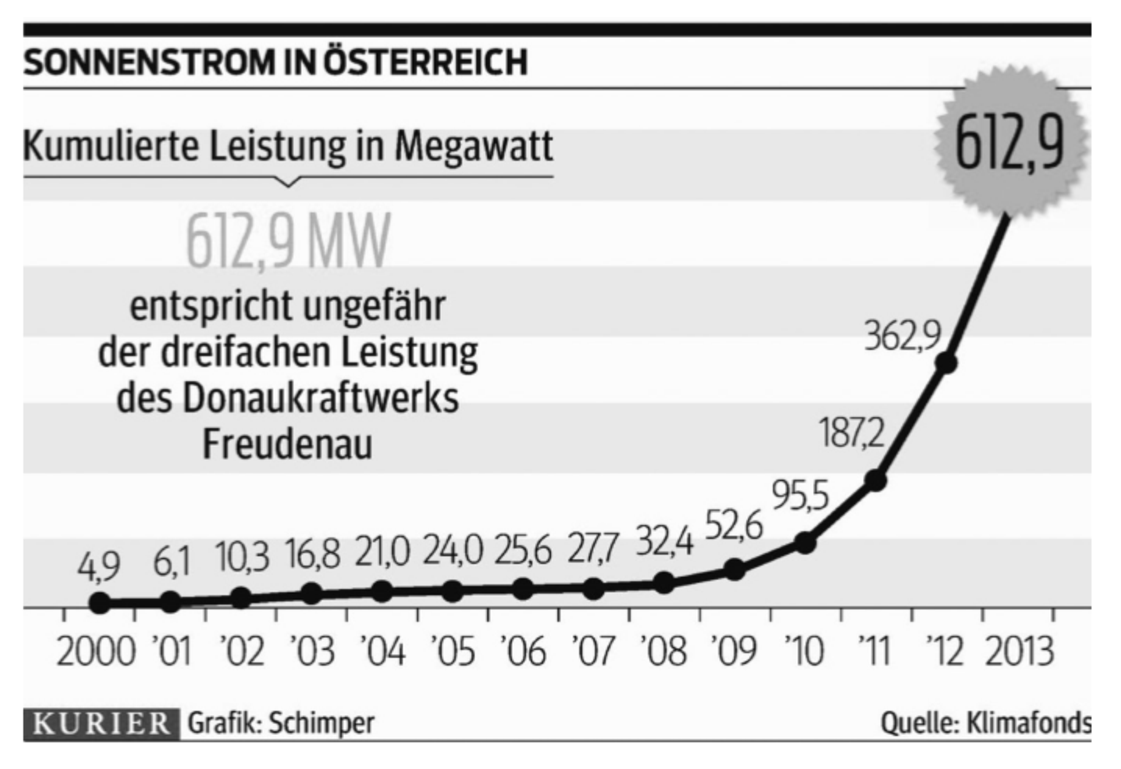
\includegraphics{../_database/Bilder/Bild69-1.eps}}
\end{center}

Es sei $t$ die Anzahl der seit dem Jahr 2000 vergangenen Jahre und $f(t)$ die in der obigen Grafik dargestellte Leistung (in MW) nach $t$ Jahren.

\subsection{Aufgabenstellung:}
\begin{enumerate}
	\item \fbox{A} Berechne und interpretiere den Differenzenquotienten $\frac{f(13)-f(0)}{13}$ im gegebenen Kontext.\leer
	
	Gib die Bedeutung des Integrals $\int^{13}_0{f(t)}$d$t$ im Hinblick auf die Erzeugung von Sonnenstrom an!
	
\item Begründe, warum die in der obigen Grafik im Zeitintervall $[9\text{ Jahre};12\text{ Jahre}]$ dargestellte Leistung (in MW) durch eine Exponentialfunktion $g$ mit der Gleichung $g(t)=a\cdot b^t$ gut angenähert werden kann!
	
	Gib den Ausdruck $\frac{f(12)-f(9)}{f(9)}+1$ mithilfe des Parameters $b$ der Funktion $g$ an!

\item Die Energiegewinnung durch eine Fotovoltaikanlage ist am größten, wenn das Sonnenlicht im rechten Winkel auf die Solarzellen trifft. 

Die optimale Neigung der Fotovoltaikmodule hängt daher vom Einfallswinkel der Sonne ab, der auf der nördlichen Erdhalbkugel am 21. Juni am größten ist.
\begin{center}
	\resizebox{0.8\linewidth}{!}{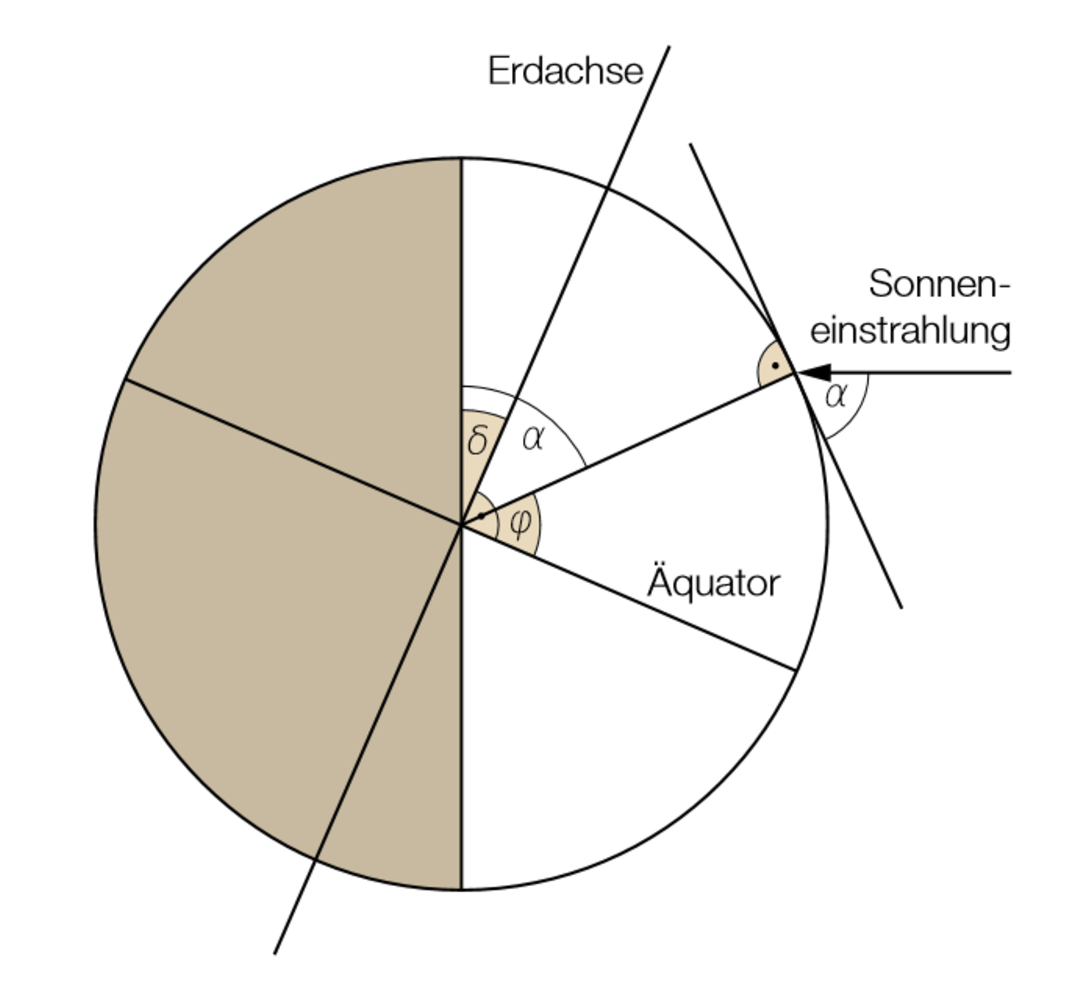
\includegraphics{../_database/Bilder/Bild69-2.eps}}
\end{center}

In der obigen Abbildung ist der Einfallswinkel $\alpha$ der Sonne am 21. Juni zu Mittag dargestellt. 

Der Winkel $\delta\approx 23,5^\circ$ gibt dabei die Neigung der Erdachse zur Bahnebene um die Sonne und der Winkel $\varphi$ die geografische Breite an.

Gib eine Formel für den Einfallswinkel $\alpha$ der Sonnenstrahlung in Abhängigkeit von der geografischen Breite $\varphi$ an!

\begin{center}
	\resizebox{0.8\linewidth}{!}{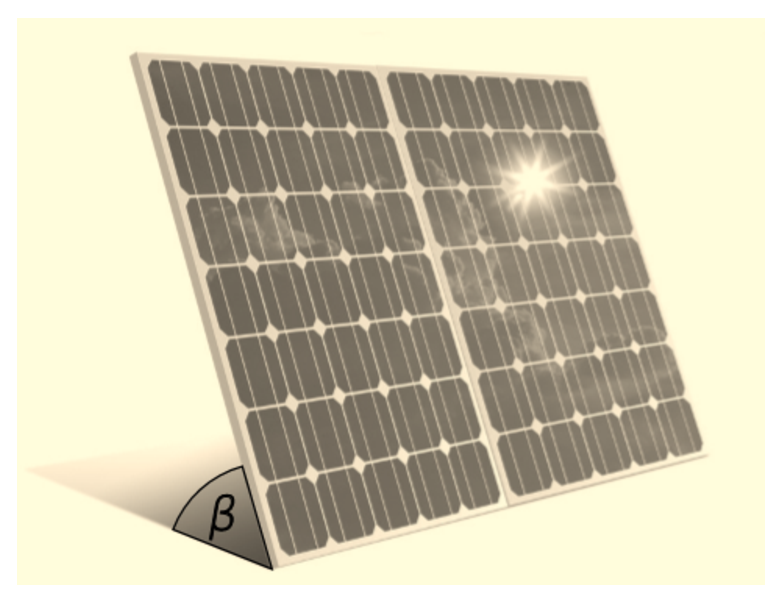
\includegraphics{../_database/Bilder/Bild69-3.eps}}
\end{center}
\begin{scriptsize}\begin{singlespace}Bildquelle: http://www.solaranlage.eu/sites/default/files/bilder/re?exionsverluste-solarmodule.jpg [14.11.2016] (adaptiert).\end{singlespace}
\end{scriptsize}

Die obige Abbildung zeigt Fotovoltaikmodule, die unter einem Winkel $\beta$ gegen die Horizontale geneigt sind. Die Solarzellen sind dabei der Sonne zugewandt.\leer

Ermittle eine Formel für den optimalen Neigungswinkel $\beta_\text{opt}$ der Fotovoltaikmodule in Abhängigkeit von demjenigen $\alpha$, bei dem das Sonnenlicht im rechten Winkel auftrifft! Gib an, wie sich dieser Winkel im Winter bzw. in höheren Breiten (d.h. bei einer Zunahme der geografischen Breite) verändert! Begründe deine Antwort!   



\end{enumerate}

\antwort{
\begin{enumerate}
	\item \subsection{Lösungserwartung:} 

$\frac{f(13)-f(0)}{13}\approx 46,8$

Im Zeitraum von 2000 bis 2013 hat die Leistung durchschnittlich um ca. 47 MW pro Jahr zugenommen.\leer
 
Das Integral gibt näherungsweise an, wie viel elektrische Energie ("`Sonnenstrom"') in den Jahren 2000 bis 2013 mithilfe von Solarzellen insgesamt erzeugt wurde.

	\subsection{Lösungsschlüssel:}
	\begin{itemize}
		\item Ein Ausgleichspunkt für die richtige Lösung und eine (sinngemäß) korrekte Interpretation.  
		
		Toleranzintervall: $[46 $MW$; 47 $MW$]$
		\item Ein Punkt für eine (sinngemäß) korrekte Interpretation.
	\end{itemize}
	
	\item \subsection{Lösungserwartung:}
			
Im Zeitintervall [9 Jahre; 12 Jahre] kommt es jährlich ungefähr zu einer Verdoppelung der Leistung.

$\frac{f(12)-f(9)}{f(9)}+1=b^3$
	
	\subsection{Lösungsschlüssel:}
	
\begin{itemize}
	\item Ein Punkt für eine (sinngemäß) richtige Begründung. 
	\item Ein Punkt für die richtige Lösung. 
\end{itemize}

\item \subsection{Lösungserwartung:}
			
$\alpha=90^\circ+\delta-\varphi=113,5^\circ-\varphi$

$\beta_\text{opt}+90^\circ+\alpha=180^\circ \Rightarrow \beta_\text{opt}=90^\circ-\alpha$\leer

Mögliche Begründung:

Da der Einfallswinkel in höheren Breiten bzw. im Winter kleiner ist, vergrößert sich die optimale Neigung der Fotovoltaikmodule.
	
	\subsection{Lösungsschlüssel:}
	
\begin{itemize}
	\item Ein Punkt für eine korrekte Formel. Äquivalente Formeln sind als richtig zu werten.
	\item Ein Punkt für eine korrekte Formel, eine korrekte Schlussfolgerung und eine (sinngemäß) korrekte Begründung. Äquivalente Formeln sind als richtig zu werten.
\end{itemize}

\end{enumerate}}
		\end{langesbeispiel}